\subsection{Interface Utilisateur et Administration du Hub}

Afin de permettre au conducteur de l'engin d'interagir avec le système de détection, de paramétrer les zones de sécurité et de consulter l'historique des alertes, une interface utilisateur a été développée. Cette interface prend la forme d'une application web développée en HTML, CSS et JavaScript, hébergée de manière autonome par le serveur web asynchrone du microcontrôleur ESP32 de l'écran tactile.

\subsubsection{Architecture logicielle et optimisations embarquées}

L'architecture de l'interface a été pensée pour pallier les contraintes de ressources du microcontrôleur :

\begin{itemize}
    \item \textbf{Une seule page :} Tous les écrans sont chargés en une seule requête initiale. Le basculement entre le menu, la configuration et l'historique se fait par manipulation du DOM, garantissant une fluidité d'affichage sans rechargement de page.
    \item \textbf{Traitement d'image Client-Side :} Lors de la configuration, l'utilisateur peut associer une photo du véhicule. Au lieu d'envoyer l'image brute à l'écran, un script JavaScript utilise l'API \texttt{Canvas} pour redimensionner l'image, lire ses pixels, et la convertir en un flux binaire brut au format \texttt{RGB565}. Les images transparentes sont également traitées et fonctionnelles. Cela épargne à l'ESP32 la charge critique de décodage d'un fichier JPEG/PNG.
\end{itemize}

\begin{figure}[H]
\centering 
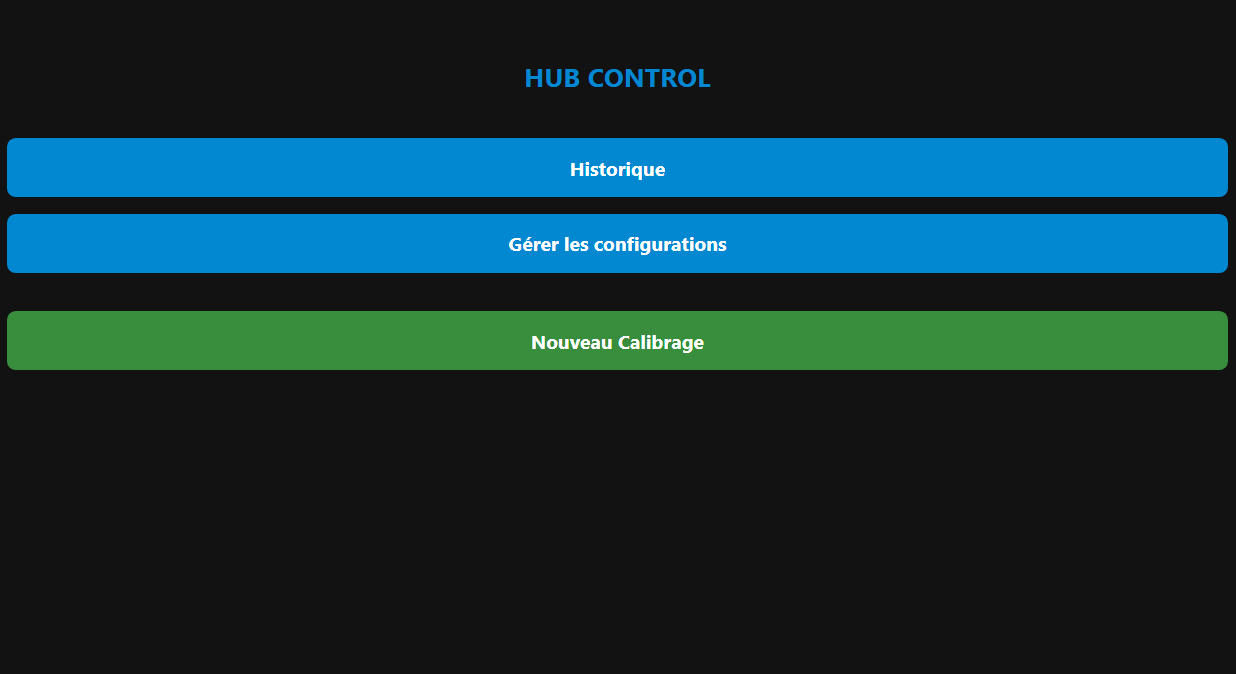
\includegraphics[width=0.6\columnwidth]{Figures/ui_home.png}
\caption[Menu principal Hub]{Menu principal de l'interface de contrôle du Hub.}
\end{figure}

\subsubsection{Étapes de Calibration de la Zone d'Exclusion}

La fonctionnalité fondamentale de l'interface réside dans son outil de calibration géométrique, permettant à l'opérateur de forger la zone de danger autour du véhicule avec précision. Ce processus s'articule en quatre étapes distinctes.

\paragraph{Étape 1 : Configuration et paramétrage matériel}
L'opérateur renseigne initialement les dimensions réelles de l'engin (longueur, largeur) ainsi que les distances séparant physiquement les ancres UWB fixées sur la machine. Cette étape est cruciale : elle permet d'établir une échelle spatiale exacte. Si l'emplacement virtuel des ancres ne correspond pas à leur disposition physique, le calcul de la position d'un ouvrier par trilatération sera projeté de manière erronée.

\begin{figure}[H]
\centering 
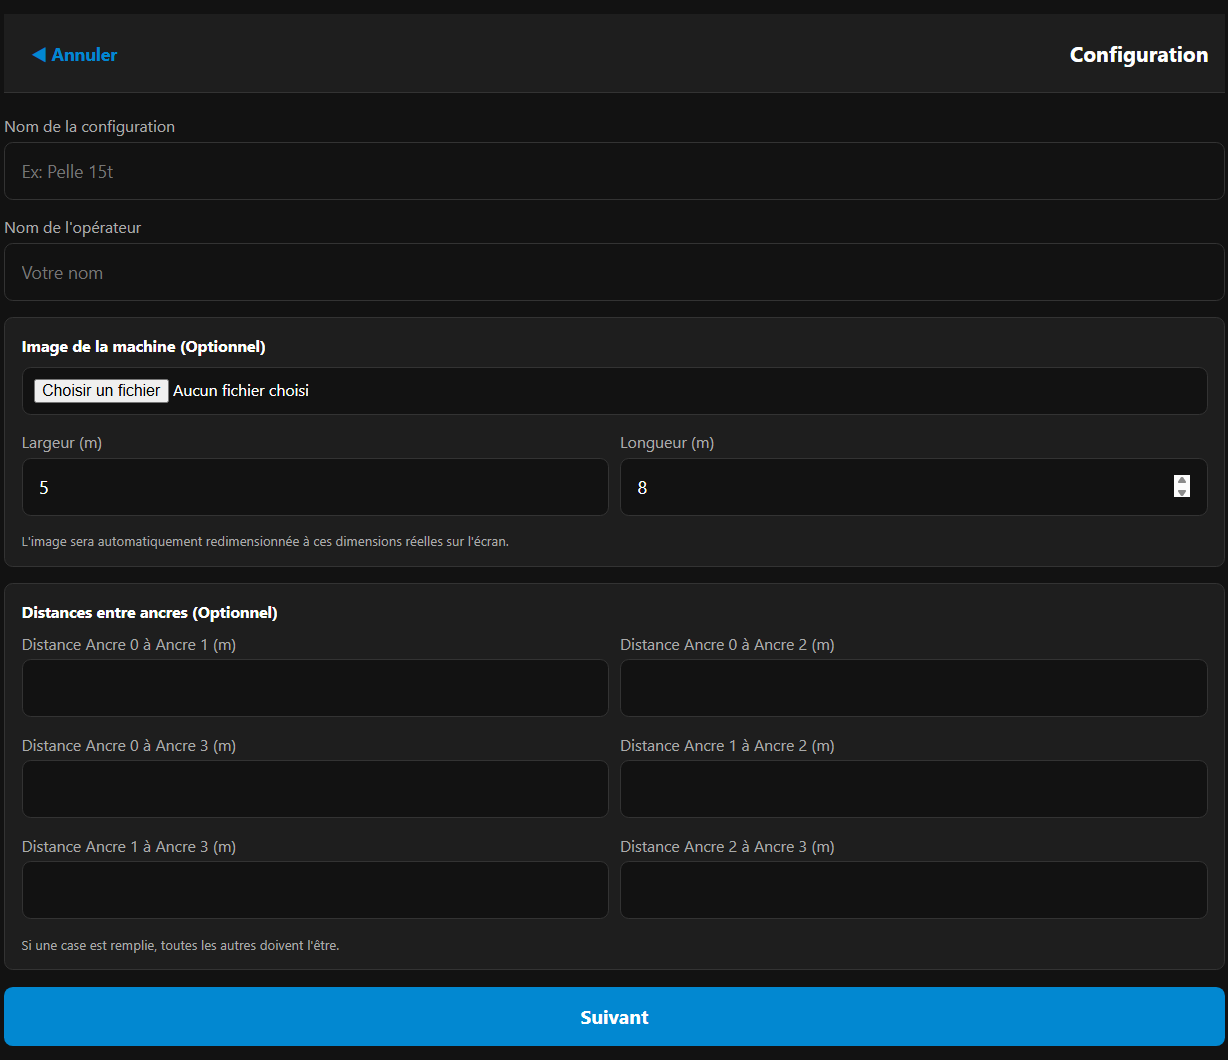
\includegraphics[width=0.7\columnwidth]{Figures/ui_setup.png}
\caption[Écran de configuration]{Vue de configuration : saisie des paramètres de l'engin et des distances inter-ancres.}
\end{figure}

\paragraph{Étape 2 : Ciblage et acquisition des données}
Une fois le véhicule configuré, le système interroge le Hub pour lister les Tags UWB actifs à proximité. L'opérateur sélectionne le Tag qu'il va porter pour effectuer sa marche de calibration. L'interface affiche alors un écran d'attente jusqu'à ce que l'utilisateur appuie sur le bouton pour terminer la calibration et que le Hub confirme la génération du polygone brut.

\begin{figure}[H]
\centering 
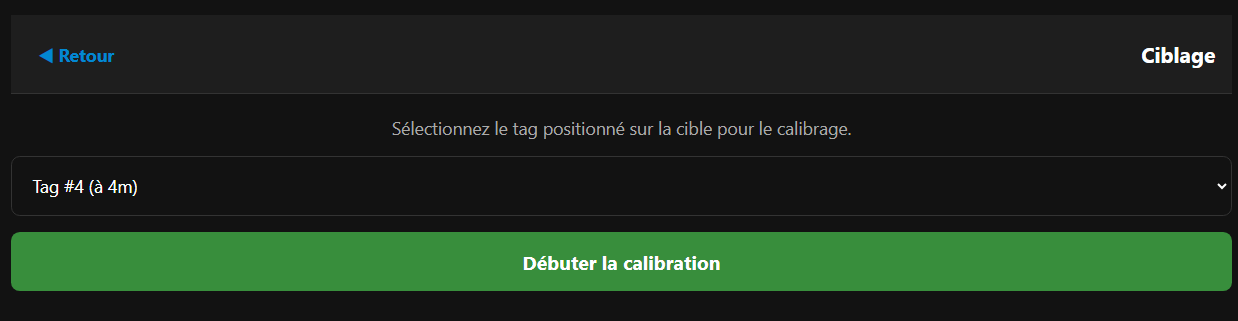
\includegraphics[width=0.7\columnwidth]{Figures/ui_acquisition.png}
\caption[Acquisition UWB]{Écrans de sélection du Tag cible et de mise en attente durant la marche de calibration.}
\end{figure}

\paragraph{Étape 3 : Alignement global par transformation affine}
Le nuage de 64 points lissé par le Hub possède une forme mathématique cohérente, mais son orientation spatiale est arbitraire, car elle dépend du point de départ de l'opérateur. L'objectif est de faire coïncider l'avant de la machine physique avec le haut de l'écran. L'utilisateur utilise un curseur rotatif et le glissement tactile pour orienter la forme sur un repère radar 2D. 

Mathématiquement, le script JavaScript applique à chaque sommet de coordonnées $(x, y)$ et à chaque capteur une transformation affine composée d'une translation de vecteur $(T_x, T_y)$ et d'une rotation d'angle $\theta$ :

\begin{equation}
\begin{pmatrix} x' \\ y' \end{pmatrix} = \begin{pmatrix} \cos \theta & -\sin \theta \\ \sin \theta & \cos \theta \end{pmatrix} \begin{pmatrix} x \\ y \end{pmatrix} + \begin{pmatrix} T_x \\ T_y \end{pmatrix}
\end{equation}

\begin{figure}[H]
\centering 
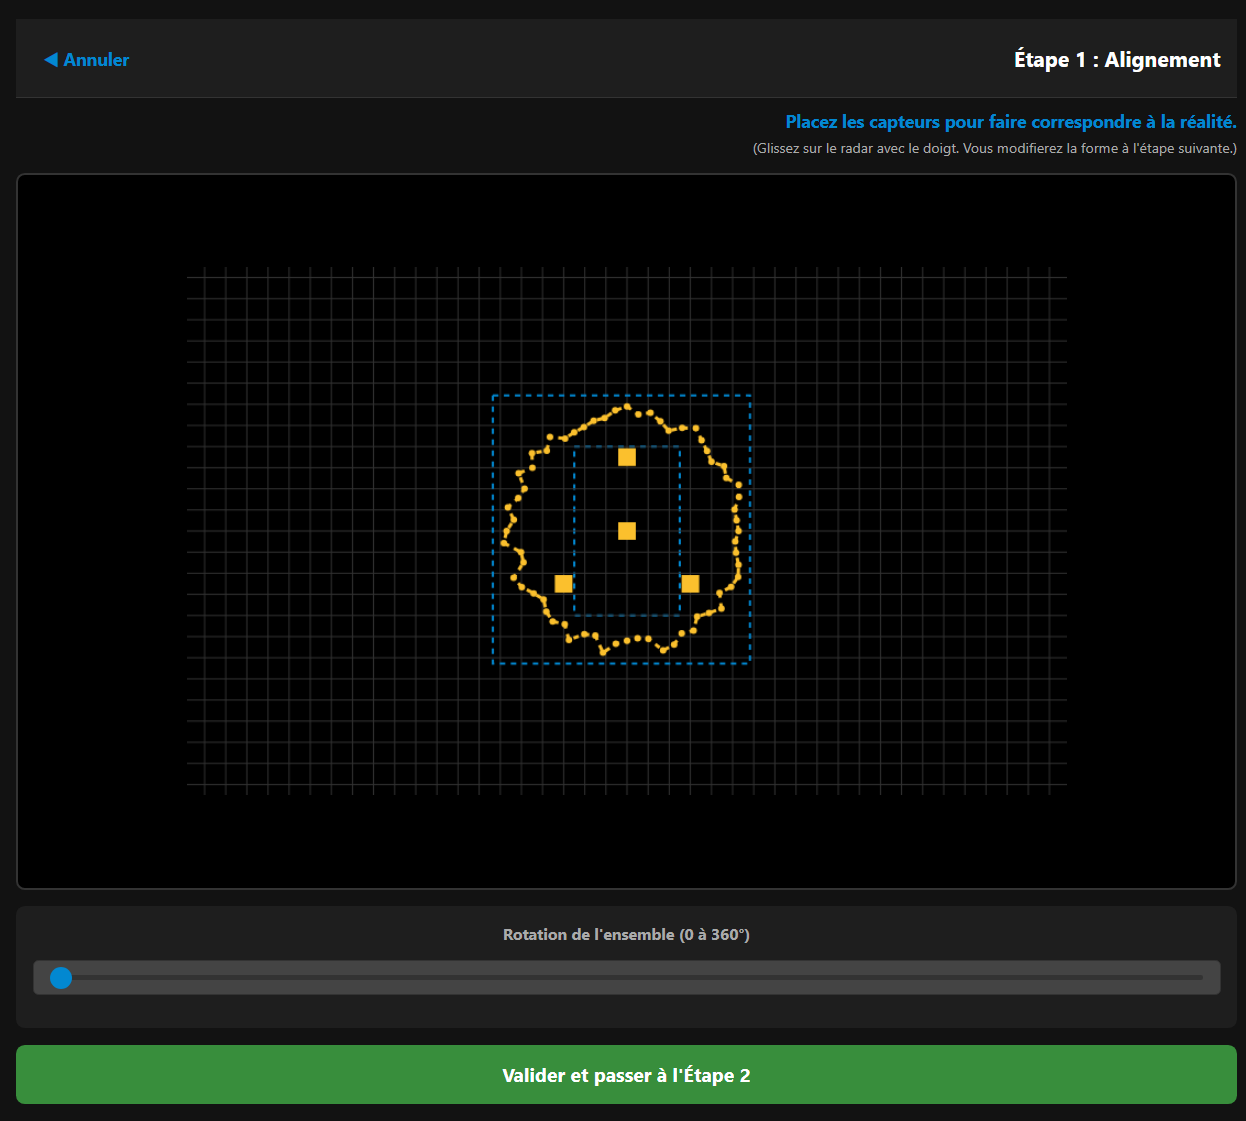
\includegraphics[width=0.7\columnwidth]{Figures/ui_align.png}
\caption[Alignement spatial]{Interface d'alignement de la zone d'exclusion par rapport au châssis de l'engin.}
\end{figure}

\paragraph{Étape 4 : Édition topologique fine (Multi-touch)}
L'imprécision inhérente à la technologie UWB peut altérer localement la géométrie de la zone d'exclusion. Un mode d'édition en plein écran gère les événements multi-touch complexes pincer pour zoomer pour le redimensionnement. L'utilisateur peut sélectionner un sommet spécifique du polygone et le déplacer individuellement. Une fonction de conversion bilatérale traduit les coordonnées de l'écran en mètres réels, garantissant une résolution centimétrique. L'altération d'un sommet entraîne la mise à jour immédiate des arêtes adjacentes.

Chaque déplacement clone l'état du polygone dans une pile en mémoire (\texttt{historyStack}), offrant une fonction d'annulation illimitée. Une fois validée, la matrice JSON normalisée est transmise au Hub via une requête HTTP POST pour enregistrement dans la mémoire Flash.

\begin{figure}[H]
\centering 
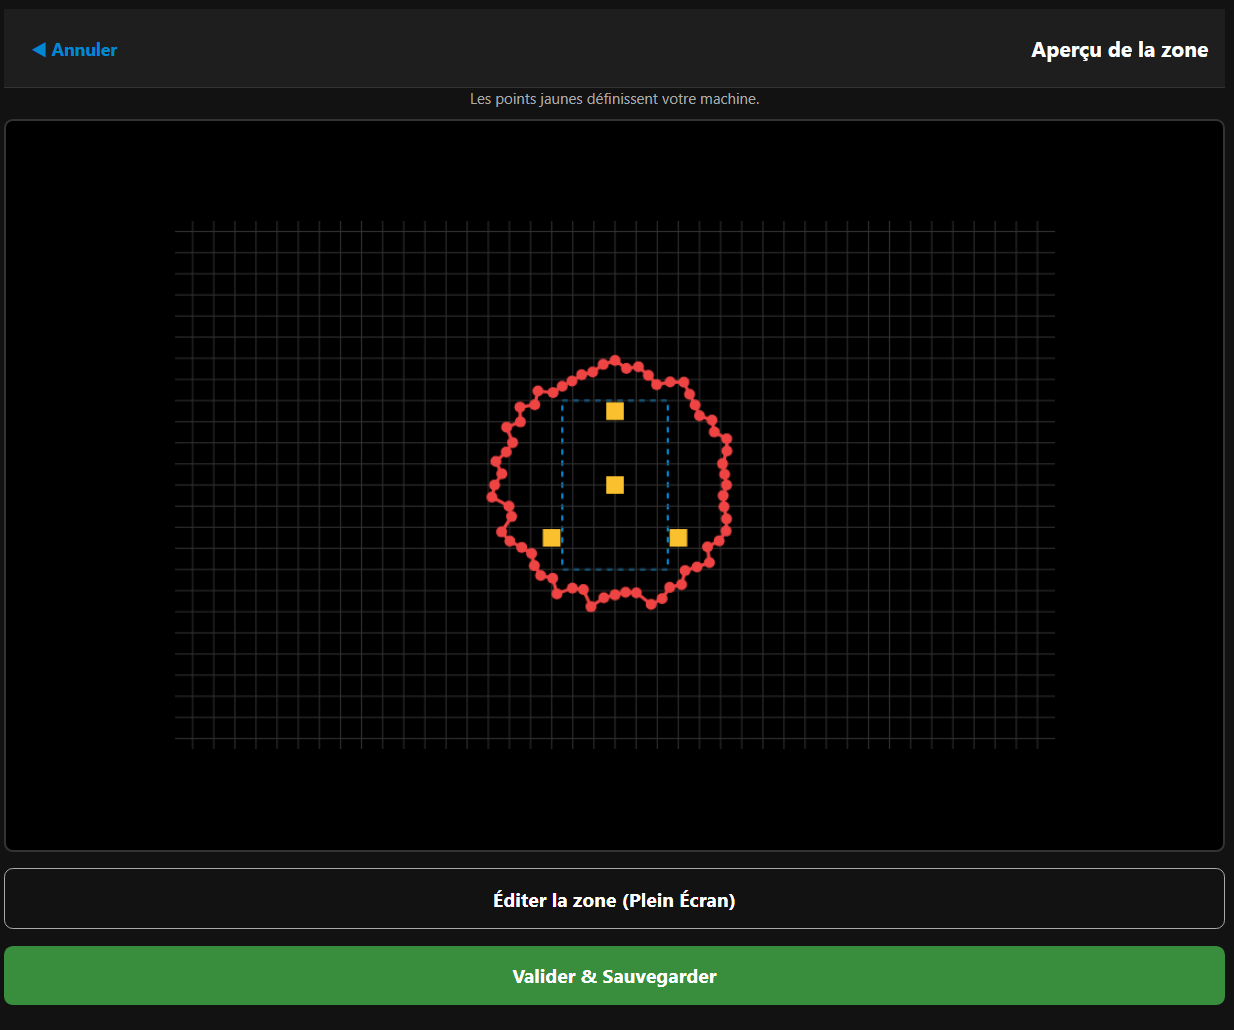
\includegraphics[width=0.8\columnwidth]{Figures/ui_edition.png}
\caption[Édition Multi-touch]{Mode d'édition plein écran avec gestion des événements tactiles pour la correction géométrique.}
\end{figure}

\subsubsection{Journalisation et Historique des Événements}

L'écran joue également le rôle de boîte noire de l'engin. L'interface propose deux journaux distincts : l'historique des modifications de configuration et le registre des alertes (franchissements de zone).

Pour assurer une fluidité totale même en cas de base de données volumineuse, l'interface exploite le concept de \emph{Virtual Scrolling}. Le script JavaScript ne génère les balises HTML \texttt{<tr>} (lignes de tableau) que pour la fraction du registre physiquement visible à l'écran. Lors du défilement, le contenu est recalculé et remplacé dynamiquement, maintenant l'empreinte mémoire du navigateur strictement constante.

\begin{figure}[H]
\centering 
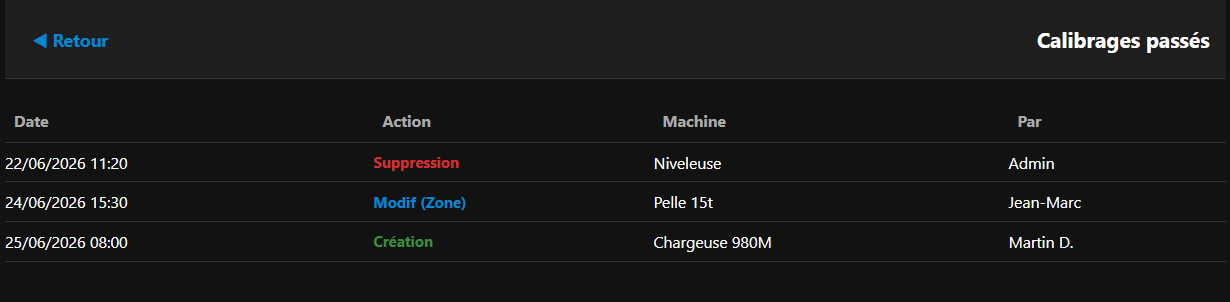
\includegraphics[width=0.7\columnwidth]{Figures/ui_history.png}
\caption[Registre des alertes]{Interface de consultation des journaux avec rendu dynamique.}
\end{figure}

\subsubsection{Architecture Backend et Gestion de l'Écran Local}

L'hébergement de cette interface web et la gestion des données asynchrones sont pilotés par le code embarqué en C++ sur l'ESP32 dédié à l'écran. Ce programme remplit trois rôles fondamentaux pour alléger la charge du processeur du Hub principal :

\paragraph{Hébergement asynchrone et mémoire SD}
Le serveur web s'appuie sur la librairie \texttt{ESPAsyncWebServer}. Afin de libérer la mémoire Flash interne, les ressources statiques de l'interface (le fichier \texttt{index.html} contenant le code de la page) ainsi que les fichiers de persistance (\texttt{calibrations.json}, \texttt{warnings.csv} sauvegardant les calibrations déjà faites et l'historique des alertes) sont stockés sur une carte mémoire micro-SD gérée via le bus \texttt{SD\_MMC}. Cela garantit une capacité d'enregistrement quasi illimitée pour les journaux d'alertes.

\paragraph{Passerelle de communication (Bridge Wi-Fi / UART)}
L'ESP32 de l'écran agit comme une passerelle réseau. Lorsqu'une requête HTTP est émise par le smartphone, le serveur web intercepte cette requête, la convertit en un objet JSON, et l'envoie au Hub via une liaison série physique (UART). Le contrôleur bascule alors dans une boucle d'écoute active pour récupérer la réponse du Hub et la transférer au client web. Ce mécanisme garantit la parfaite étanchéité entre la couche réseau utilisateur et la couche calcul du Hub.

\paragraph{Rendu graphique local (LVGL)}
En parallèle du serveur web, la boucle principale pilote l'affichage physique de l'écran tactile via la librairie graphique \texttt{LVGL}. Le microcontrôleur lit en temps réel les états d'alarme transmis par le Hub. Si une intrusion est détectée, le programme déclenche asynchrone un clignotement rouge des indicateurs visuels locaux, assurant au conducteur de l'engin un avertissement visuel absolu et immédiat, totalement indépendant de la connexion Wi-Fi de l'application web.